\documentclass[12pt,compress,english,utf8,t]{beamer}
\usepackage[english]{babel}
\usepackage{calc}
\usepackage{ragged2e,wasysym,multicol,mathtools}
\usepackage[protrusion=true,expansion=true]{microtype}
\hypersetup{colorlinks=true}

\graphicspath{{images/}}

\DeclareSymbolFont{extraup}{U}{zavm}{m}{n}
\DeclareMathSymbol{\varheart}{\mathalpha}{extraup}{86}

\title[{Exploring hypercomputation with the ef{}fective topos}]{Exploring hypercomputation \\ $\varheart$ with the ef{}fective topos $\varheart$}
\author[Ingo Blechschmidt]{\textcolor{white}{Ingo Blechschmidt \\ \scriptsize University of Augsburg \\ February 8th, 2017}}
\date[2017-02-08]{}

%\usetheme{Warsaw}
\useinnertheme[shadow=true]{rounded}
\useoutertheme{split}
\usecolortheme{orchid}
\usecolortheme{whale}
\setbeamerfont{block title}{size={}}

\useinnertheme{rectangles}

\usecolortheme{seahorse}
\definecolor{mypurple}{RGB}{150,0,255}
\setbeamercolor{structure}{fg=mypurple}
\definecolor{myred}{RGB}{150,0,0}
\setbeamercolor*{title}{bg=myred,fg=white}
\setbeamercolor*{titlelike}{bg=myred,fg=white}

\usefonttheme{serif}
\usepackage[T1]{fontenc}
\usepackage{libertine}
%\usepackage{mathpazo}

\renewcommand{\_}{\mathpunct{.}\,}
\newcommand{\BB}{\mathbb{B}}
\newcommand{\M}{\mathcal{M}}
\newcommand{\R}{\mathrm{R}}
\newcommand{\NN}{\mathbb{N}}
\newcommand{\RR}{\mathbb{R}}
\newcommand{\Eff}{\mathrm{Eff}}
\newcommand{\TM}{\mathrm{TM}}
\newcommand{\STM}{\mathrm{STM}}
\newcommand{\RW}{\mathrm{RW}}
\newcommand{\lambdaC}{\lambda\mathrm{C}}
\newcommand{\defeq}{\vcentcolon=}
\newcommand{\Set}{\mathrm{Set}}

\newcommand{\code}[1]{%
  \begin{center}%
    \setlength{\fboxrule}{1pt}%
    \setlength{\fboxsep}{8pt}%
    {\fbox{\parbox{0.81\textwidth}{#1}}}%
  \end{center}%
}

\newcommand{\explanation}[2]{
  #1 \\
  \qquad means: \\[0.4em]
  \qquad\qquad \begin{minipage}{0.84\textwidth}
  #2
  \end{minipage}
}

\newcommand{\explanationspoiler}[3]{
  \explanation{#1}{#2} \\[0.4em]
  \qquad\qquad\qquad #3
}

\newcommand{\fmini}[2]{%
  \setlength{\fboxrule}{2pt}%
  \setlength{\fboxsep}{-3pt}%
  \usebeamercolor[fg]{item}\fbox{\usebeamercolor[fg]{normal text}\parbox{#1}{\begin{center}#2\end{center}}}}

\setbeamertemplate{navigation symbols}{}

\setbeamertemplate{title page}[default][colsep=-1bp,rounded=false,shadow=false]
\setbeamertemplate{frametitle}[default][colsep=-2bp,rounded=false,shadow=false,center]

\newcommand{\hil}[1]{{\usebeamercolor[fg]{item}{\textbf{#1}}}}
\setbeamertemplate{frametitle}{%
  \vskip1em%
  \leavevmode%
  \begin{beamercolorbox}[dp=1ex,center]{}%
      \usebeamercolor[fg]{item}{\textbf{\Large \insertframetitle}}
  \end{beamercolorbox}%
}

\setbeamertemplate{footline}{%
  \leavevmode%
  \hfill%
  \begin{beamercolorbox}[ht=2.25ex,dp=1ex,right]{}%
    \usebeamerfont{date in head/foot}
    \insertframenumber\,/\,\inserttotalframenumber\hspace*{1ex}
  \end{beamercolorbox}%
  \vskip0pt%
}

\newcommand{\backupstart}{
  \newcounter{framenumberpreappendix}
  \setcounter{framenumberpreappendix}{\value{framenumber}}
}
\newcommand{\backupend}{
  \addtocounter{framenumberpreappendix}{-\value{framenumber}}
  \addtocounter{framenumber}{\value{framenumberpreappendix}}
}

\newcommand{\partslide}[5]{{\usebackgroundtemplate{\begin{minipage}{\paperwidth}\vspace*{#3}\centering\includegraphics[#2]{#1}\end{minipage}}
\begin{frame}
  \centering
  \bigskip\bigskip

  \Huge \hil{Part #4}

  \bigskip
  \Large\textbf{#5}
  \par
\end{frame}}}


\setbeameroption{show notes}
%\setbeamercolor{note page}{bg=red!30}
\setbeamertemplate{note page}[plain]

\begin{document}

% http://www.ufointernationalproject.com/wp-content/uploads/2015/11/a23.jpg
{\usebackgroundtemplate{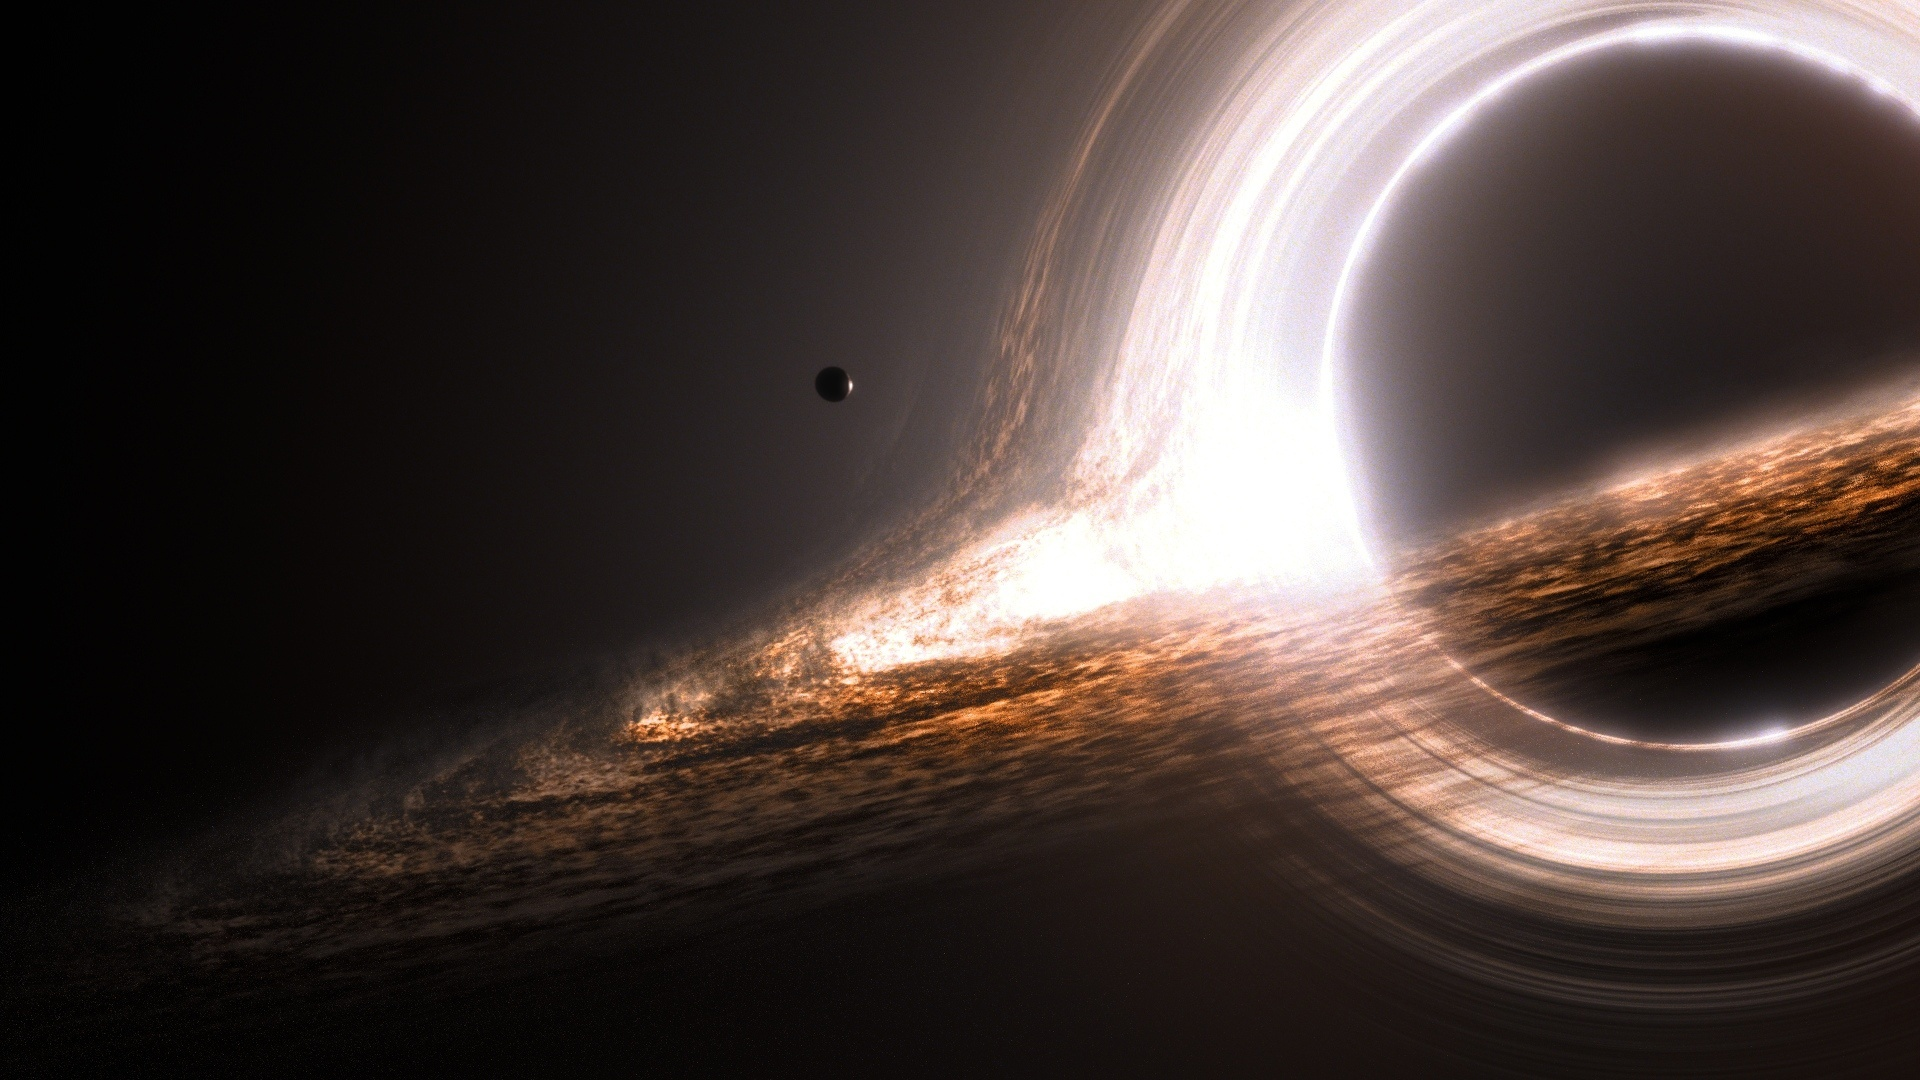
\includegraphics[height=\paperheight]{interstellar}}
\frame{\vspace*{11em}\titlepage}}
\setcounter{tocdepth}{2}
\frame{\tableofcontents}


\section[Ordinal numbers]{Crash course on ordinal numbers}

\partslide{infinite-queue}{width=0.4\paperwidth}{4.5cm}{I}{A crash course on ordinal numbers}

\note{
  The \href{https://en.wikipedia.org/wiki/Ordinal_number}{Wikipedia article on
  ordinal numbers} is a good starting point. For the purposes of this talk,
  it suffices to have some intuitive grasp of the ordinal number line:
  \[ 0,\ 1,\ 2,\ \ldots,\ \omega,\ \omega + 1,\ \omega + 2,\ \ldots,\ \omega\cdot2,\ \omega\cdot2 + 1,\ \ldots \]
}


\section{(Super) Turing machines}

\partslide{turing-machine}{width=0.5\paperwidth}{4.5cm}{II}{(Super) Turing machines}


\subsection[TM]{Bacics on Turing machines}

\newcommand{\portrait}[4]{\begin{column}{#3\textwidth}\centering\includegraphics[height=#4\textheight]{#1}\\{\scriptsize #2\par}\end{column}}

\begin{frame}{Basics on Turing machines}
  \begin{itemize}
    \item Turing machines are idealised computers operating on an \hil{infinite
    tape} according to a \hil{finite list} of rules.
    \item The concept is astoundingly robust.
    \item A subset of~$\NN$ is \hil{enumerable by a Turing machine} if and only
    if it's a $\Sigma_1$-set.
  \end{itemize}

  \bigskip
  \begin{columns}[t]
    \begin{column}{0.095\textwidth}\end{column}
    \portrait{alan-turing}{Alan Turing \\ (* 1912, † 1954)}{0.27}{0.35}
    \portrait{imitation-game}{worth watching}{0.27}{0.35}
    \portrait{alison-bechdel}{Alison Bechdel \\ (* 1960)}{0.27}{0.35}
    \begin{column}{0.095\textwidth}\end{column}
  \end{columns}
\end{frame}

\note{
  \begin{itemize}
    \item\justifying There are explicit examples for Turing machines with a
    very small number of states for which their halting behaviour is unknown.
    There are other examples for which their halting behaviour is independent
    of standard Zermelo--Fraenkel set theory.

    \item Besides Turing machines, there are alternative models for
    computation, for instance lambda calculus and register machines. For
    functions~$\NN \to \NN$, these models all yield the same notion of
    computabitility. For higher-order functions, where the domain is a set of
    functions, the models typically differ in which functions they deem
    computable.
  \end{itemize}
}

\note{\begin{itemize}
  \item\justifying A set~$M \subseteq \NN$ is \emph{enumerable by a Turing
  machines} (or \emph{recursively enumerable}) if and only if there is a Turing
  machine which outputs all the elements of~$M$ (in an arbitrary order, using
  some fixed encoding).

  \item A set~$M \subseteq \NN$ is a~$\Sigma_1$-set if and only if there is
  a~$\Sigma_1$-formula~$\varphi$ of first-order arithmetic containing exactly one free
  variable such that $M = \{ n \in \NN \,|\, \varphi(n) \}$.
  A formula~$\varphi$ is a~$\Sigma_1$-formula if and only if it is of the form
  \[ \exists m_1\_ \exists m_2\_ \ldots \exists m_k\_ \heartsuit, \]
  where the existential quantifiers range over the natural numbers and no
  further unbounded quantifiers (of any kind) may appear in the
  subformula~$\heartsuit$.
\end{itemize}}

\note{\justifying
  There is also a deep link between computability and number
  theory: A set~$M \subseteq \NN$ is enumerable by a Turing machine if and only
  if it is a \emph{diophantine set}, that is of the form
  \[ M = \{ n \in \NN \,|\, \text{the eq.\@ $f(n,x_1,\ldots,x_m) = 0$
  has a solution} \}, \]
  where $f$ is a polynomial with integral coefficients and ``solution'' means
  integral solution.
}

\note{\justifying
  Just as \emph{Logicomix: An Epic Search for Truth} illustrates the
  foundational quest in mathematics (starring Cantor, Hilbert, Gödel, Turing,
  and others), the graphic novel \emph{The Thrilling Adventures of Lovelace and
  Babbage} explores the history of programmable computers.\bigskip

  \begin{columns}[t]
    \begin{column}{0.13\textwidth}\end{column}
    \portrait{logicomix}{}{0.37}{0.4}
    \portrait{lovelace-babbage}{}{0.37}{0.4}
    \begin{column}{0.13\textwidth}\end{column}
  \end{columns}
}


\subsection[STM]{Bacis on super Turing machines}

\begin{frame}{Super Turing machines}
  With super Turing machines, the time axis is more interesting:
  \begin{itemize}
    \item normal: $0,\ 1,\ 2,\ \ldots$
    \item super:\phantom{rl} $0,\ 1,\ 2,\ \ldots,\ \omega,\ \omega + 1,\ \ldots,\ \omega\cdot2,\ \omega\cdot2
    + 1,\ \makebox[\widthof{R}][l]{$\ldots\ldots\ldots\ldots\ldots\ldots$}$
  \end{itemize}
  \bigskip

  On reaching a limit ordinal time step like~$\omega$ or~$\omega \cdot 2$,
  \begin{itemize}
    \item the machine is put into a designated state,
    \item the read/write head is moved to the start of the tape, and
    \item the tape is set to the ``lim sup'' of all its previous contents.
  \end{itemize}

  \bigskip
  \begin{columns}[t]
    \begin{column}{0.03\textwidth}\end{column}
    \portrait{joel-david-hamkins}{Joel David Hamkins}{0.23}{0.3}
    \portrait{mathoverflow}{MathOverflow}{0.38}{0.3}
    \portrait{phantom}{Andy Lewis}{0.23}{0.3}
    \begin{column}{0.03\textwidth}\end{column}
  \end{columns}
\end{frame}

\note{\justifying
  We can imagine a super Turing machine to take one second for
  its first computational step, half a second for the next step, a quarter of a
  second for the step after that, and so on. After two seconds, the machine
  will have completed infinitely many steps.

  \medskip
  {\centering\includegraphics[width=0.35\textwidth]{ordinal-omega-squared}\par}
  \medskip

  \scriptsize
  The fine print: This visual illustration only
  works for those ordinals which can be embedded into the ordinary real number
  line~$\RR$. These are exactly the countable ordinals, those ordinals for
  which the set of predecessors is countable. Luckily, the interesting
  behaviour of a super Turing machine always takes place in the realm of
  countable ordinal numbers (even though this is not a requirement we put on
  super Turing machines a priori).\par
}

{\usebackgroundtemplate{\includegraphics[height=\paperheight]{who-wants-to-be-a-millionaire}}
\begin{frame}{A question to you}
  \centering
  What's the behaviour of this super Turing machine?

  \code{In the start state and the limit state, check whether the current cell contains a ``1''.
  \begin{itemize}
    \item If yes, then stop.
    \item If not, then flash that cell: set it to ``1'', then reset it to ``0''. Then
    unremittingly move the head rightwards.
  \end{itemize}}
  \pause
  This machine halts after time step~$\omega^2$.
  \bigskip

  \parbox{0.72\textwidth}{\centering\hil{Super Turing machines can break out of (some kinds of) infinite loops.}\par}
  \par
\end{frame}}

\note{
  There is an \href{https://asciinema.org/a/66yqvm1qjormhj6tgl2wzyvu8}{ASCII
  video} of a run of that machine.
}


\subsection[Power]{The power of super Turing machines}

\begin{frame}{What can super Turing machines do?}
  \begin{itemize}
    \item Everything ordinary Turing machines can do.
    \item Verify number-theoretic statements.
    \item Decide whether a given ordinary Turing machine halts.
    \item Simulate super Turing machines.
    \item Decide $\Pi_1^1$- and $\Sigma_1^1$-statements:
    \begin{itemize}
      \item ``For any function $\NN \to \NN$ it holds that \ldots''
      \item ``There is a function $\NN \to \NN$ such that \ldots''
    \end{itemize}
  \end{itemize}

  \visible<2>{\hil{But:} Super Turing machines can't compute all functions
  and can't write arbitrary 0/1-sequences to the tape.}

  \begin{center}
    \scalebox{0.1}{\input{images/nonwellfounded-tree.pdf_t}}
  \end{center}
\end{frame}


\subsection[Outlook]{Outlook on the larger theory}

{\usebackgroundtemplate{\includegraphics[height=\paperheight]{lost-melody}}
\begin{frame}{Fun facts}
  \begin{itemize}
    \item Any super Turing machine either halts or gets caught in an
    unbreakable infinite loop after \hil{countably many steps}.
    \item An ordinal number~$\alpha$ is \hil{clockable} iff there is a super
    Turing machine which halts precisely after time step~$\alpha$.
    \begin{itemize}
      \item Speed-up Lemma: If $\alpha + n$ is clockable, then so is $\alpha$.
      \item Big Gaps Theorem
      \item Many Gaps Theorem
      \item Gapless Blocks Theorem
    \end{itemize}
    \item \hil{Lost Melody Theorem:} There are 0/1-sequences which a super Turing
    machine can recognise, but not write to the tape.
  \end{itemize}
\end{frame}}

\note{\begin{itemize}
  \item\justifying In view of the fact that super Turing machines always halt
  at countable ordinal numbers (if they halt at all), the ability of super
  Turing machines to decide~$\Pi_1^1$- and~$\Sigma_1^1$-statements is even more
  astounding.

  \item That there are at least some ordinal numbers which are not clockable,
  can be seen by a simple cardinality argument: There are only countably many
  super Turing machines, but a proper class worth of ordinal numbers.

  \item The Big Gaps Theorem states: For any clockable ordinal~$\alpha$ there
  is a gap of length~$\geq \alpha$ in the clockable ordinals.
\end{itemize}}

\note{\begin{itemize}
  \item\justifying The \href{https://arxiv.org/abs/math/9808093}{seminal paper}
  introducing super Turing machines is a joy to read. It contains the
  statements and proofs of all the cited theorems.

  \item I'm using the adjectives ``super'', ``hyper'', and ``infinite-time''
  interchangably.
\end{itemize}}

\section{The ef{}fective topos}

\partslide{topos-horses}{width=\paperwidth}{4.95cm}{III}{The ef{}fective topos}

\note{\justifying
  For any model~$\mathcal{M}$ of computation, such as Turing machines~($\TM$), super
  Turing machines~($\STM$), or lambda calculus~($\lambdaC$), there is an
  associated \emph{ef{}fective topos} $\mathrm{Eff}(\mathcal{M})$. Formally, a
  topos is a certain kind of category; intuitively, a topos is an alternate
  mathematical universe in which the usual laws of logic may not necessarily
  hold.
  \bigskip

  The standard universe, in which most of mathematics happens, is the
  topos~$\Set$.
  \bigskip

  One can even employ machines of the real physical world as the
  ``model''~$\mathcal{M}$ used for constructing the ef{}fective topos~($\RW$).
  Statements about the resulting topos are then statements about the real
  world instead of formal mathematical statements.
  \par
}

\subsection[First steps]{First steps in the ef{}fective topos}

\begin{frame}{The ef{}fective topos}
  \begin{itemize}
    \item ``$1 + 1 = 2$.''

    \visible<2->{True in $\Set$, true in~$\Eff(\TM)$.}
    \medskip

    \item ``Any number is either prime or not.''

    \visible<3->{Trivially true in $\Set$, nontrivially true in~$\Eff(\TM)$.}
    \medskip

    \item ``Any function $\NN \to \NN$ is either the zero function or not.''

    \visible<4->{Trivially true in $\Set$, false in~$\Eff(\TM)$.}
    \medskip

    \item ``Any function $\NN \to \NN$ is computable by a Turing machine.''

    \visible<5->{False in $\Set$, trivially true in~$\Eff(\TM)$.}
    \medskip

    \item ``Any function $\RR \to \RR$ is continuous.''

    \visible<6->{False in $\Set$, nontrivially true in~$\Eff(\TM)$.}
  \end{itemize}
\end{frame}

\begin{frame}{First steps in the ef{}fective topos}
  \small
  \explanation{$\Eff(\TM) \models \text{``For any number~$n$ there is a prime~$p
  > n$.''}$}{There is a Turing machine which reads a number~$n$ as input and outputs a
  prime number~$p > n$.}
  \bigskip

  \only<1>{
    \centering
    \hil{``Realisability Theory''}
    \par
  }
  \pause

  \explanation{\mbox{$\Eff(\TM) \models \text{``Any number has a prime factor
  decomposition.''}$}}{There is a Turing machine which reads a number $n$ as input and
  outputs a list of primes, the product of which is~$n$.}
  \bigskip
  \pause

  \explanation{$\Eff(\TM) \models \text{``Any number is either prime or not
  prime.''}$}{There is a Turing machine which reads a number $n$ as input and outputs
  YES or NO depending on whether $n$ is prime or not.}
\end{frame}


\subsection[Constructive logic]{The wonder of constructive logic}

\subsubsection{What's true in alternate toposes?}

\begin{frame}{What's true in alternate toposes?}
  \hil{Metatheorem:} If a statement has a \hil{constructive proof},
  then it holds in \hil{any topos}.
  \bigskip

  Constructive logic is like classical logic, except we don't suppose the
  \hil{law of excluded middle} (LEM), which says:
  \begin{itemize}
    \item ``Any statement is either true or not true.''
    \item ``If a statement is \emph{not not} true, then it's true.''
  \end{itemize}

  \bigskip\centering
  \includegraphics[width=0.2\textwidth]{lem}
  \par
\end{frame}

\note{\begin{itemize}
  \item\justifying The technical term for ``constructive logic'' is
  ``intuitionistic logic''. ``Constructive logic'' or even ``constructive
  mathematics'' is more of an umbrella term which might mean any of several
  related, but not equivalent systems.

  \item The law of excluded middle is the axiom which allows us to
  argue by contradiction. But the word ``contradiction'' is still allowed in
  constructive mathematics; see below.

  \item The proof of the metatheorem is constructive.
\end{itemize}}


\subsubsection{Nonconstructive proofs}

\begin{frame}{Nonconstructive proofs}

  {\centering\includegraphics[scale=0.20]{pythagoras}\par}

  \hil{Theorem.} There are \hil{irrational} numbers~$x$ und~$y$ such that~$x^y$ is rational.
  \medskip

  \pause
  \hil{Proof.} Either~$\sqrt{2}^{\sqrt{2}}$ is rational or not.
  \begin{enumerate}
    \item In the first case we are done.
    \item In the second case we set~$x \defeq \sqrt{2}^{\sqrt{2}}$ and~$y \defeq
    \sqrt{2}$. Then~$x^y = \sqrt{2}^{\sqrt{2} \cdot \sqrt{2}} =
    \sqrt{2}^2 = 2$ is rational.
  \end{enumerate}
\end{frame}

\note{\justifying
  The proof is nice and short. However, after having seen the proof, we are still not able
  to give an example of irrational numbers~$x,y$ such that~$x^y$ is rational!
  The proof was \emph{non-constructive}. If we want to extract explicit
  witnesses from the proof, the proof has to be constructive, such as this one:

  \begin{quote}Set~$x \defeq \sqrt{2}$ and~$y \defeq \log_{\sqrt{2}} 3$.
  Then~$x^y = 3$ is rational. The proof that~$y$ is irrational is even easier
  than the proof that~$\sqrt{2}$ is irrational.\end{quote}

  It turns out that from all the axioms of classical logic, exactly one is
  responsible for non-constructivity: the law of excluded middle.
  \par
}


\subsubsection[Praise]{Appreciating constructive logic}

\begin{frame}{Appreciating constructive logic}
  At first sight, dropping the law of excluded middle looks like a sad thing
  to do. It's a useful axiom! However:

  \begin{itemize}\justifying
    \item The axiom is not needed as often as one would think.
    \item The abstinence is good for your mental hygiene.
    \item Constructive logic allows for finer distinctions.
    \item From constructive proofs one can mechanically extract programs which
    witness the proved statements.
    \item \hil{Dropping the law of excluded middle allows to add curious unconvential axioms.}
  \end{itemize}
\end{frame}

\note{\justifying
  We're used to immediately cancel double negations. Since that's
  constructively not possible, we have to exercise a bit of linguistic
  caution:

  \begin{itemize}
  \item\justifying
  \emph{Proof of a negated statement (constructively acceptable):}
  We want to verify~$\neg\psi$. Assume that~$\psi$ holds. Then \ldots,
  that's a contradiction. Therefore~$\neg\psi$.

  This is a constructively valid argument, since in constructive (and
  classical) logic~$\neg\psi$ is defined as the implication~$(\psi \Rightarrow
  \bot)$, where~$\bot$ is the formal logical symbol for falsity, a
  contradiction.

  \item \emph{Proof by contradiction (constructively not acceptable a priori):}
  We want to verify~$\varphi$. Assume that~$\varphi$ is false. Then \ldots,
  that's a contradiction. Therefore~$\varphi$ holds.

  The constructively valid part of this argument only shows that~$\varphi$ does
  \emph{not not} hold: $\neg\neg\varphi$.\par
  \end{itemize}
}

\note{\justifying
  Several years ago a video showing Kate Moss consuming drugs surfaced. From
  the video it was clear that the drugs were either of some type~$A$ or of some
  type~$B$, but there was no direct evidence for either type. Kate Moss was
  not prosecuted; in this sense, the judicial system operated on
  constructive logic. Check out
  \href{http://blog.sigfpe.com/2008/06/drugs-kate-moss-and-intuitionistic.html}{Dan
  Piponi's blog post about this topic}.
  \par
}

\note{\justifying
  Constructive logic allows for finer distictions than classical logic.
  For instance, if we know that the key to our apartment has to be somewhere in
  the apartment (since we used it to enter last night) but we can't find it
  right now, we can constructively only justify
  \[ \neg\neg( \exists x\_ \text{the key is at position $x$} ), \]
  not the stronger statement
  \[ \phantom{\neg\neg(} \exists x\_ \text{the key is at position
  $x$},\phantom{)} \]
  because for justifying the stronger statement we'd had to give an explicit
  witness of the existential statement (the position of the key).
  \bigskip

  \scriptsize
  (Both examples do not quite work, since constructive mathematics is (like
  classical mathematics) indifferent to our personal state of knowledge.)
  \par
}

\note{\justifying
  Constructive mathematicians do \emph{not} claim that the law of excluded
  middle is false (that is, that its negation holds). In fact, some instances
  of the law of excluded middle are true intuitionistically: For example one
  can show by induction that any natural number is zero or is not zero.
  Constructive mathematicians simply don't suppose that the law of excluded
  holds generally.
  \bigskip

  The analogous statement about real numbers does not have a constructive
  proof. This is linked with a familiar fact from programming: It's unbeseeming
  to compare floating point numbers for equality, while there is no such
  problem with comparing integers.
  \par
}

\note{\justifying
  Philosophers don't only study what's \emph{true}, but also what \emph{should
  be true}, what's \emph{possible}, what's \emph{necessary}, what
  somebody \emph{knows} or somebody \emph{believes}. This is formalised using
  \emph{modal operators}.
  \bigskip

  Mathematicians don't need to envy that greater scope: In constructive
  mathematics there is too a multitude of modal operators. Double negation is
  the most prominent example.\bigskip

  Andrej Bauer gave a very insightful talk about the merits of constructive
  mathematics at the Institute for Advanced Study. His talk is a joy to watch!
  \begin{itemize}
    \item \href{https://www.youtube.com/watch?v=21qPOReu4FI}{video}
    \item
    \href{http://www.ams.org/journals/bull/0000-000-00/S0273-0979-2016-01556-4/S0273-0979-2016-01556-4.pdf}{accompanying
    article}
  \end{itemize}
}

\subsection[Tautologies]{Ef{}fective content of classical tautologies}

\subsubsection[Functions]{Equality of functions}

\begin{frame}{LEM for equality of functions}
  \explanationspoiler{$\Eff(\TM) \models \begin{minipage}[t]{0.7\textwidth}
  ``Any function~$f : \NN \to \NN$ is either the zero function or
  not.''\\[-0.7em]\end{minipage}$}{There is a Turing machine which reads the
  source of a Turing machine~$M$, which computes a function $\NN \to \NN$, as input, and finds out whether~$M$ always yields zero or not.}{That's false.}
  \bigskip
  \pause

  The statement is true in~$\Eff(\STM)$, the ef{}fective topos associated to
  super Turing machines.
\end{frame}


\subsubsection[Halting]{The halting problem}

\begin{frame}{LEM for the halting problem}
  \explanationspoiler{$\Eff(\TM) \models \text{``Any Turing machine halts or
  doesn't halt.''}$}{There is a Turing machine which reads the source of a Turing machine~$M$
  as input and finds out whether $M$ halts or not.}{That's false.}
  \bigskip
  \pause

  The statement is true in~$\Eff(\STM)$.
\end{frame}


\subsubsection[Reals]{Equality of real numbers}

\begin{frame}{LEM for equality of real numbers}
  \justifying
  The statement
  \[ \text{``Every real number is either zero or not zero.''} \]
  is in constructive logic equivalent to
  \[ \text{``Every Turing machine halts or doesn't halt.''}, \]
  so it's not true in~$\Eff(\TM)$, but in~$\Eff(\STM)$.
  \bigskip
  \pause

  For a Turing machine~$M$ consider the real number~$0.000\ldots$ whose~$n$'th
  decimal digit is a one iff~$M$ halts after step~$n$.
  \bigskip

  For a real number~$x$ consider the Turing machine which searches the digits
  of~$x$ for a nonzero digit.
  \par
\end{frame}

\note{\justifying
  Is the statement true in~$\Eff(\RW)$, the ef{}fective topos associated to
  machines of the real world? That means: Is it possible to build a halting
  oracle in the real world? A machine which reads the description of a Turing
  machine and then outputs whether the Turing machine halts or not?
  \bigskip

  Since this is not about the halting problem for machines of the real world
  (which is not decidable by machines of the real world, by the
  \href{https://en.wikipedia.org/wiki/Halting_problem}{usual argument}), but
  only about the halting problem for Turing machines, the answer \emph{might}
  be ``yes''. Tricks using black holes and relativistic time dilation might
  be possible.\bigskip

  More details on~$\Eff(\RW)$ are contained in the very accessible book chapter
  \href{http://math.andrej.com/wp-content/uploads/2014/03/real-world-realizability.pdf}{Intuitionistic
  Mathematics and Realizability in the Physical World} by Andrej Bauer.\par
}


\subsubsection[Markov]{Markov's principle}

\begin{frame}{Markov's principle}
  \explanationspoiler{$\Eff(\TM) \models \begin{minipage}[t]{0.7\textwidth}
  ``For any function~$f : \NN \to \NN$ which is not the zero function,
  there is a number~$n \in \NN$ such that~$f(n) \neq
  0$.''\\[-0.7em]\end{minipage}$}{There is a Turing machine which reads the source of a
  Turing machine~$M$, which computes a function~$\NN \to \NN$ which is not the zero
  function, as input and outputs a number~$n$ such that~$M(n)$ is not
  zero.}{\pause That's true! By unbounded search.}
\end{frame}


\subsubsection[Choice]{The axiom of choice}

\begin{frame}{The axiom of choice}
  \justifying
  A set~$X$ ist \hil{projective} if and only if, for any set~$Y$ and
  any formula~$\varphi(x,y)$ with parameters~$x \in X$, $y \in Y$ it holds that:
  \begin{center}\parbox{0.75\textwidth}{
    If for any~$x \in X$ there is an element~$y \in Y$ such
    that~$\varphi(x,y)$, then
    there is a map~$f : X \to Y$ such that~$\varphi(x,f(x))$ for all~$x \in X$.
  }\end{center}
  \[ \forall x \in X\_ \exists y \in Y\_ \varphi(x,y) \ \Longrightarrow\
    \exists f \in Y^X\_ \forall x \in X\_ \varphi(x,f(x)) \]
  The \hil{axiom of choice} of classical mathematics states that any set is
  projective.

  \begin{itemize}
    \item In~$\Eff(\TM)$ the set~$\NN$ is projective, but~$\NN^\NN$ is not.
    \item In~$\Eff(\STM)$ the sets~$\NN$ and~$\NN^\NN$ are projective.
    \item In~$\Eff(\RW)$ the set~$\NN^\NN$ is projective if black boxes are
    possible.
  \end{itemize}
\end{frame}

\note{\justifying
  Finite sets are projective even in constructive mathematics.
  \bigskip

  By~$\NN^\NN$, we mean the set of all functions~$\NN \to \NN$.
  \par
}

\note{\justifying
  \scriptsize
  A good way to convince oneself that the axiom of choice is indeed a
  nontrivial statement is to look at what the statement ``$\NN^\NN$ is
  projective'' means in~$\Eff(\TM)$. It means that the statement
  \begin{center}\parbox{0.86\textwidth}{
    There is a Turing machine~$M$ which reads the description of a Turing
    machine~$P$, which computes a function~$f : \NN \to \NN$, as input and
    outputs an element~$M(P) \in Y$ together with a witness
    of~$\varphi(f,M(P))$.
  }\end{center}
  implies
  \begin{center}\parbox{0.86\textwidth}{
    There is a computable map~$g$ from the set of computable maps~$f : \NN \to
    \NN$ to the set~$Y$ such that for all such functions~$f$ the
    statement~$\varphi(f,g(f))$ holds in~$\Eff(\TM)$.
  }\end{center}

  On first sight, this implications seems to be true:
  It seems that one could define the looked-for map~$g$ to be simply the map computed by~$M$.
  But that doesn't necessarily work: If~$f : \NN \to \NN$ is a map which is computed
  by a Turing machine~$P$, then the element~$M(P)$ might depend on the concrete
  realisation of~$f$ by the machine~$P$. Different implementations of~$f$ by
  different Turing machines~$P'$ might yield different elements~$M(P')$.
  Therefore the resulting ``map''~$g$ might be multi-valued, so not a proper
  map.
  \par
}


\subsubsection[Imp.\@]{Searching uncountable sets}

\begin{frame}{Searching uncountable sets}
  \begin{center}\parbox{0.91\textwidth}{
    ``For any function $f : \NN \to \BB$ from numbers to~$\BB = \{0,1\}$
    there either exists a number~$n$ such that $f(n) = 1$ or there is no such number.''
  }\end{center}
  This statement is false in~$\Eff(\TM)$.
  \bigskip
  \bigskip

  \begin{center}\parbox{0.91\textwidth}{
    ``For any function $P : \BB^\NN \to \BB$ from infinite lists of booleans to booleans,
    there either exists a list~$x$ such that $P(x) = 1$ or there is no such list.''
  }\end{center}
  \pause
  This statement is true in~$\Eff(\TM)$!
\end{frame}

\note{\justifying
  It's somewhat miraculous that the countable set~$\NN$ can not be searched,
  but the uncountable set
  \[ \BB^\NN = \prod_{n=0}^\infty \BB = \{ (x_0,x_1,\ldots) \} \]
  can. There is a deeper topological reason for this fact: The space~$\BB^\NN$
  is compact (by Tychonoff's theorem) while~$\NN$ is not.
  \bigskip

  Details are available in a
  \href{http://math.andrej.com/2007/09/28/seemingly-impossible-functional-programs/}{blog
  post by Martín Escardó}.\par
}


\subsubsection[Church--Turing]{The Church--Turing thesis}

\begin{frame}{The Church--Turing thesis}
  \justifying
  The \hil{Church--Turing thesis} states:
  \bigskip

  {\centering\parbox{0.82\textwidth}{If a function $f : \NN \to
  \NN$ is computable in the real world, then it's also computable by a Turing
  machine.}\par}
  \bigskip

  \explanationspoiler{$\Eff(\TM) \models \begin{minipage}[t]{0.7\textwidth}
  ``Any function~$f : \NN \to \NN$ is computable by a
  Turing machine.''\\[-0.7em]\end{minipage}$}{There is a Turing machine which reads the source of a
  Turing machine computing a function~$f : \NN \to \NN$ as input and
  outputs the source of a Turing machine which computes~$f$.}{That's trivial,
  echo the input back to the user.}
  \bigskip
  \pause

  In~$\Eff(\STM)$ the statement is false.
\end{frame}

\note{\justifying
  The statement ``any function~$\NN \to \NN$ is computable by a Turing
  machine'' is the \emph{formal Church--Turing thesis}. It is wrong in the
  standard topos~$\Set$.
  \bigskip

  The meaning of the formal Church--Turing thesis in~$\Eff(\STM)$ is: ``There
  is a super Turing machine which reads the source of a super Turing machine
  computing a function~$f : \NN \to \NN$ as input and outputs the source of an
  \emph{ordinary} Turing machine which computes~$f$.'' This is false.
  \bigskip

  The statement is also false in~$\Eff(\lambdaC)$, the ef{}fective topos
  associated to lambda calculus. This is because of different calling
  conventions; a higher-order lambda term has no access to the syntactic
  structure of a passed argument.
  \par
}

\note{\justifying
  Whether the formal Church--Turing thesis holds in~$\Eff(\RW)$, the
  ef{}fective topos associated to machines of the real world, depends on the
  nature of computation in the real world.\par
}

\note{\justifying
  The topos~$\Eff(\TM)$ is a nice context for computer science, since in it
  uncomputable functions are not present.
  By contrast, in classical mathematics, there are many functions which are not
  computable.  Two of the most famous ones are the ``halting predicate'' and
  the ``Busy Beaver function'':
  \begin{align*}
    H(n) &= \begin{cases}
      1, & \text{if the~$n$'th Turing machine halts,} \\
      0, & \text{otherwise.}
    \end{cases} \\
    BB(n) &= \text{maximal number of steps which a halting Turing machine} \\
    &\qquad\quad\text{with $n$ states performs before halting.}
  \end{align*}
  Can't we use exactly the same definitions in the ef{}fective topos, thereby
  contradicting the theorem that all functions in the ef{}fective topos are
  computable?\par
}

\note{\justifying
  The apparent paradox is resolved in the following way. The theorem only states
  that total functions~$\NN \to \NN$ are computable. However, to verify
  that~$H$ and~$BB$ are indeed such total functions, the law of excluded middle
  is necessary:
  \bigskip

  For~$H$, in order to be able to make the case distinction.
  \bigskip

  For~$BB$, because implicitly the lemma that every ``subfinite'' set of natural
  numbers contains a maximal element was used. This lemma depends on the law of
  excluded middle.\par
}


\subsubsection[Cont.\@]{Automatic continuity}

\begin{frame}{Automatic continuity}
  \justifying
  The following statement is wildly \hil{false} in~$\Set$:
  \[ \text{``Every function $f : \RR \to \RR$ is continuous.''} \]
  A function~$f$ is \hil{continuous} if and only if, for calculating~$f(x)$ to
  finitely many digits, finitely many digits of~$x$ suffice.\par

  \centering
  \includegraphics[width=0.5\textwidth]{plot-1-en}
  \includegraphics[width=0.5\textwidth]{plot-2-en}
  \par
  \pause

  \justifying
  \hil{True} in $\Eff(\TM)$. \pause
  True in~$\Eff(\RW)$, if private communication channels are possible and
  only finitely many computational steps can be executed in finite time.\par
\end{frame}

\note{\justifying
  Don't there obviously exist discontinuous functions? Like the sign function?
  \[ \mathrm{sgn} : \RR \to \RR, \quad
    x \mapsto \begin{cases}
      -1, & \text{if $x < 0$,} \\
      0,  & \text{if $x = 0$,} \\
      1,  & \text{if $x > 0$.}
    \end{cases}
  \]
  Without the presence of the law of excluded middle, the situation is not so
  trivial: Without LEM, one cannot show that this rule
  defines a total function~$\RR \to \RR$, because without LEM, the lemma
  ``every real number is either $< 0$, $= 0$, or $> 0$'' can't be shown.
  (This lemma implies the weaker statement that any real number is either zero
  or not zero. We've already seen that this statement is false in~$\Eff(\TM)$.)
  \medskip

  Without LEM, the rule only defines a function~$M \to \RR$, where~$M =
  \{ x \in \RR \,|\, x < 0 \vee x = 0 \vee x > 0 \}$.
  \par
}

\note{\justifying
  The real numbers can be constructed in several different ways, for instance
  using Cauchy sequences or Dedekind cuts. Because the axiom of dependent
  choice holds in~$\Eff(\TM)$,~$\Eff(\STM)$, and~$\Eff(\RW)$, all those
  constructions coincide.\bigskip

  Externally, a real number in any of these toposes is given by a machine which
  produces coherent, arbitrarily good approximations. For instance, one could
  ask such a machine for approximations which are correct to three, seven, or
  ten digits and obtain the answers
  \[ 3.1417777777, \quad 3.1415926777, \quad\text{and}\quad 3.1415926535. \]
  Machines which compute different, but equally good approximations represent
  the same real number.\par
}

\note{\justifying
  \scriptsize
  The fine print: By ``correct to~$n$ digits'' we mean ``distance at
  most~$10^{-n}$ to the true value''. We don't literally refer to the first~$n$
  digits after the decimal point (which aren't well-defined anyway,
  $0.999\ldots = 1$).
  \medskip

  For instance, the approximation~$0.999$ of the number~$1$ is correct to three
  digits while~$0.998$ is only correct to two digits.\par
}

\note{\justifying\scriptsize
  The meaning of the statement ``all functions~$\RR \to \RR$ are continuous''
  in the ef{}fective topos is: There is a machine~$M$ which takes

  \vspace{-1.2em}
  \begin{enumerate}
    \item\justifying a machine~$A$ which computes a function~$f : \RR \to \RR$, \\[-1.4em]
    \item a machine~$X$ which represents a real number~$x$, and \\[-1.4em]
    \item a natural number~$n$
  \end{enumerate}
  \vspace{-1.2em}

  as inputs and outputs a natural number~$m$ with the following property:
  For any real number~$\tilde x$ which is the same as~$x$ to~$m$ digits,
  the numbers~$f(x)$ and~$f(\tilde x)$ are the same to~$n$ digits.\smallskip

  In the case of real world machines, one can proceed as follows to construct
  such a machine~$M$. Given~$A$,~$X$, and~$n$, the machine~$M$ should call~$A$
  with a slight variant~$X'$ of~$X$: The machine~$X'$ should exhibit the same
  input/output behaviour as~$X$, but on each call~$X'$ should tell~$M$ using a
  private communication channel how many digits were asked for. Since~$X'$ has
  the same input/output behaviour as~$X$, the machine~$A$ is bound by contract
  to react to~$X'$ in the same way as it reacts to~$X$.\smallskip

  If the real world is such that only finitely many computational steps can be performed in finite time,
  then~$M$ can determine a suitable number~$m$ as follows: It just
  has to wait till~$A$ has computed~$f(x)$ to~$n$ digits. It can then look at
  its log to see how many digits of~$x$ $A$ used for the computation. For any
  number~$\tilde x$ which is equal to~$x$ to this amount of digits, the
  number~$f(\tilde x)$ produced by~$A$ is the same as~$f(x)$ to~$n$ digits.\par
}

\note{\justifying
  Not a fan of real numbers? The same phenomenon is visible at other types, for
  instance for functions~$f : \BB^\NN \to \BB$, where~$\BB = \{ 0,1 \}$ as
  before. Such a function is continuous if and only if, for any~$x \in \BB^\NN$
  (that is, any function~$x : \NN \to \BB$) there exists a number~$m$ such
  that~$f(x)$ depends only on the first~$m$ values of~$x$.\bigskip

  In~$\Eff(\TM)$, the statement ``every function~$f : \BB^\NN \to \BB$ is
  continuous'' is true.\par
}


% \begin{document}


\subsubsection[Sizes]{Curious size phenomena}

\begin{frame}{Curious size phenomena}
  \only<1-2>{
    There is no surjection~$\NN \to \NN^\NN$; the set~$\NN^\NN$ of
    functions~$\NN \to \NN$ is much larger than~$\NN$.
    \bigskip

    A corollary in classical logic is: There is no injection~$\NN^\NN \to \NN$.
    This expresses the same intuition about the relative sizes.
    \bigskip

    \begin{columns}[t]
      \begin{column}{0.13\textwidth}\end{column}
      \portrait{surjection}{a surjection \\ ``$X$ is greater than $Y$''}{0.37}{0.25}
      \portrait{injection}{an injection \\ ``$X$ is smaller than $Y$''}{0.37}{0.25}
      \begin{column}{0.13\textwidth}\end{column}
    \end{columns}
    \bigskip

    \pause
    In~$\Eff(\STM)$, there \hil{is such an injection}.
  }

  \only<3>{
    \begin{columns}[t]
      \begin{column}{0.13\textwidth}\end{column}
      \portrait{surjection}{a surjection \\ ``$X$ is greater than $Y$''}{0.37}{0.25}
      \portrait{injection}{an injection \\ ``$X$ is smaller than $Y$''}{0.37}{0.25}
      \begin{column}{0.13\textwidth}\end{column}
    \end{columns}
    \bigskip

    \explanation{$\Eff(\STM) \models \text{``There exists an injection~$\NN^\NN \to
    \NN$.''}$}{There is a super Turing machine which inputs the source of a
    super Turing machine~$A$ computing a function~$\NN \to \NN$ and
    outputs a number~$n(A)$ such that~$n(A) = n(B)$ if and only if~$A$ and~$B$
    compute the same function.}
  }

  \only<4>{
    \explanation{$\Eff(\STM) \models \text{``There exists an injection~$\NN^\NN \to
    \NN$.''}$}{There is a super Turing machine which inputs the source of a
    super Turing machine~$A$ computing a function~$\NN \to \NN$ and
    outputs a number~$n(A)$ such that~$n(A) = n(B)$ if and only if~$A$ and~$B$
    compute the same function.}

    This statement is witnessed by following super Turing machine:
    \code{
      Read the source of a super Turing machine~$A$ from the tape.
      Simulate all super Turing machines in a dovetailing fashion.
      As soon a machine is found which has the same input/output behaviour
      as~$A$, output the number of this machine and halt.
    }
  }
\end{frame}

\note{\justifying
  The number computed by that super Turing machine depends on the input/output
  behaviour of~$A$, the chosen order of all super Turing machines, and on
  details on the way the interleaving simulation works -- but it does
  \emph{not} depend on the implementation of~$A$.\medskip

  The search terminates since there is at least one super Turing machine which
  halts on any natural number input and shows the same input/output behaviour
  as~$A$: $A$ itself.\medskip

  This injection was
  \href{http://math.andrej.com/2011/06/15/constructive-gem-an-injection-from-baire-space-to-natural-numbers/}{found
  by Andrej Bauer}.\par
}

\note{\justifying
  Just because it is so nice, here is a constructively valid proof that there
  is no surjection~$\NN \to \NN^\NN$:\bigskip

  Let~$s : \NN \to \NN^\NN$ be an arbitrary map. We want to verify that~$s$ is
  not surjective. For this, we consider the map~$f : \NN \to
  \NN$ given by
  \[ f(n) \vcentcolon= s(n)(n) + 1. \]
  This element~$f \in \NN^\NN$ is not in the image of~$s$: If there existed a
  number~$m$ such that~$s(m) = f$, then
  \[ s(m)(m) = f(m) = s(m)(m) + 1. \]
}

\note{\justifying
  When thinking about size issues, it's important to not mix up the external
  and internal point of view -- else one encounters \emph{Skolem's paradox}:
  How is it possible that~$\Eff(\TM)$ doesn't contain a surjection~$\NN \to
  \NN^\NN$, even though the object~$\NN^\NN$ of the ef{}fective topos contains
  only computable functions and there are only countably many of those?\bigskip

  It's true that the underlying set of the object~$\NN^\NN$ of~$\Eff(\TM)$ is
  countable, so that there is a surjection (even bijection)~$\NN \to
  \NN^\NN$.\bigskip

  But any such surjection is either not computable, therefore not contained
  in~$\Eff(\TM)$, or is computable, but in a way that there is no computable
  witness of its surjectivity. Therefore~$\NN^\NN$ looks like an uncountable
  set from the internal point of view~$\Eff(\TM)$, just as Cantor's theorem
  predicts.\par
}


\subsection{Wrapping up}

{\usebackgroundtemplate{\begin{minipage}{\paperwidth}\vspace*{4.95cm}\centering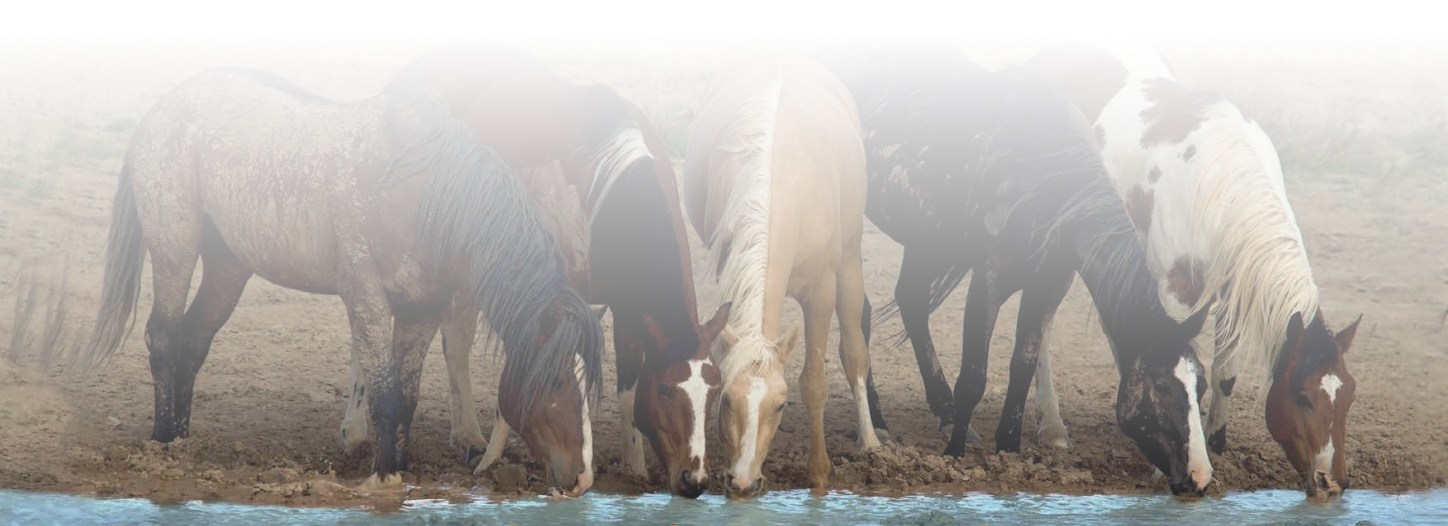
\includegraphics[width=\paperwidth]{topos-horses}\end{minipage}}
\begin{frame}{Wrapping up}
  \begin{itemize}
    \item Ef{}fective toposes are a good vehicle for studying the nature of computation.
    \item Ef{}fective toposes build links between constructive mathematics and programming.
    \item Toposes allow for curious dream axioms.
    \item Toposes also have a geometric flavour: points, subtoposes, continuous maps
    between toposes.
  \end{itemize}
  \pause

  \centering
  \bigskip
  \hil{\textcolor{white}{There is more to mathematics \\
  than the standard topos.}}
  \par
\end{frame}}

\note{\justifying
  Any topos has a \emph{largest dense subtopos}. The largest dense subtopos
  of~$\Eff(\TM)$ is~$\Set$, the standard topos. It is related to the
  \emph{double negation modality}.\bigskip

  For instance, the statement ``for any number~$n$ there is a prime~$p > n$''
  holds in~$\Eff(\TM)$ for the nontrivial reason that there exists a Turing
  machine which can find arbitrarily large prime numbers. The weaker statement
  ``for any number~$n$ there is \emph{not not} a prime~$p > n$'' holds
  in~$\Eff(\TM)$ as well, but doesn't require a witness by a machine.
  \bigskip

  If one prefixes all occurences of~``$\exists$'' and~``$\vee$'' in a formula~$\varphi$
  with~``$\neg\neg$'''s, then it loses its computational content. This modified
  formula holds in~$\Eff(\TM)$ if and only if the original formula holds
  in~$\Set$.\par
}

\note{\justifying
  For any \emph{oracle}~$L$ (as studied in computer science), the ef{}fective
  topos associated to Turing machines with access to~$L$ is a subtopos
  of~$\Eff(\TM)$. It too corresponds to a certain modal operator.
  \par
}

\note{\justifying
  In the \emph{smooth topos}, employed in synthetic differential geometry, the
  following statement holds:

  \code{Axiom of microaffinity: For any function~$f : \Delta \to \RR$,
  where~$\Delta = \{ \varepsilon \in \RR \,|\, \varepsilon^2 = 0 \}$, there
  exists a unique pair~$(a,b)$ of real numbers such that
  \[ f(\varepsilon) = a + b \varepsilon \]
  for all~$\varepsilon \in \Delta$.}
}

\end{document}
